\documentclass[a4paper]{article}
\usepackage[margin=3.5cm]{geometry}
\usepackage{amsmath,amsfonts,amssymb,amsthm}
\usepackage{thmtools, thm-restate}
\usepackage{graphicx}
\usepackage{dsfont}
\usepackage{hyperref}
\usepackage{datetime}
\usepackage{float}

\newdateformat{monthyeardate}{\monthname[\THEMONTH] \THEYEAR}

\author{Jeroen van Riel}
\date{\monthyeardate\today}
\title{Policy Gradient Reinforcement Learning}

\begin{document}

\maketitle

\section{Stationary distribution for finite episodes}

For some fixed policy $\pi$ and initial state distribution $h$, we consider the
underlying \textit{induced Markov chain} over states. Because we are working with finite
episodes, the induced state process is a Markov chain with absorbing states.
%
We want to analyze how often states are visited on average, over multiple episodes.
%
To see what \textit{on average} means here, imagine that we link together separate
episodes to create a regular Markov chain without absorbing states, in the
following way: from each final state, we introduce state transitions to the
initial states according to distribution $h$, see also Figure~\ref{fig:episodic_MC}. Furthermore,
we will write $S_{t}^{(i)}$ to denote the state at step $t$ of episode $i$.

Consider an absorbing Markov chain with transition matrix
\begin{align*}
  P_{xy} = \sum_{a} \pi(a | x) p(y | x, a) .
\end{align*}
There are $t$ transient states and $r$ absorbing states, so $P$ can be written
as
\begin{align*}
  P = \begin{pmatrix}
        Q & R \\
        \mathbf{0} & I_{r}
      \end{pmatrix} ,
\end{align*}
where $Q$ is a $t$-by-$t$ matrix, $R$ is a nonzero $t$-by-$r$ matrix, $I_{r}$ is
the $r$-by-$r$ identify matrix and $\mathbf{0}$ is the zero matrix.
%
Observe that $(Q^{k})_{xs}$ is the probability of reaching state $s$ in $k$
steps without being absorbed, starting from state $x$. Hence, the expected
number of visits to state $s$ without being absorbed, starting from state $x$,
is given by
\begin{align*}
  \eta(s | x) := \sum_{k=0}^{\infty} (Q^{k})_{xs} .
\end{align*}
%
Writing this in matrix form $N_{xs} = \eta(s | x)$, we can use the following
property of this so-called Neumann series, to obtain
\begin{align*}
  N = \sum_{k=0}^{\infty} Q^{k} = {(I_{t} - Q)}^{-1} .
\end{align*}
Now we can derive two equivalent equations
\begin{align*}
  N = (I_{t} - Q)^{-1} \iff
  \begin{cases}
    N (I_{t} - Q) = I_{t} \iff N = I_{t} + NQ ,
    \quad  \text{ or }  \\
    (I_{t} - Q) N = I_{t} \iff N = I_{t} + QN . \\
  \end{cases}
\end{align*}
%
Expanding the first equation in terms of matrix entries $N_{xs} = \eta(s | x)$
gives
\begin{align*}
  \eta(s | x) &= \mathds{1}\{ x = s \} + \sum_{y}  \eta(y | x) Q_{ys} \\
  &= \mathds{1}\{ x = s \} +  \sum_{y}\eta(y | x) \sum_{a} \pi(a | y) p(y | x, a)
\end{align*}
and similarly, the second equation gives
\begin{align*}
  \eta(s | x) &= \mathds{1}\{ x = s \} + \sum_{y} Q_{xy} \eta(s | y) \\
  &= \mathds{1}\{ x = s \} +  \sum_{a} \pi(a | x) \sum_{y} p(y | x, a) \eta(s | y)
\end{align*}
%
Now since the initial state is chosen according to distribution $h$, the
expected number of visits $\eta(s)$ to state $s$ in some episode is given by
\begin{align*}
  \eta(s) = \sum_{x} h(x) \eta(s | x) ,
\end{align*}
or written in matrix form $\eta = hN$, where $\eta$ and $h$ are row vectors.
%
Therefore, we can also work with the equations
\begin{align*}
  \begin{cases}
  hN = h + hNQ , \quad \text{ or } \\
  hN = h + hQN ,
  \end{cases}
\end{align*}
which are generally called \textit{balance equations}.
% or written in terms of matrix entries, respectively,
% \begin{align*}
%   \begin{cases}
%   \eta(s) = h(s) + \sum_{x} h(x) \sum_{y} \eta(y|x) \sum_{a} \pi(a|y)p(s|y, a) , \text{ or } \\
%   \eta(s) = h(s) + \sum_{x} h(x) \sum_{a} \pi(a | x) \sum_{y} p(y | x, a) \eta(s | y) .
%   \end{cases}
% \end{align*}
By writing the first variant as $\eta = h + \eta Q$ and expanding the matrix
multiplication, we obtain
\begin{align*}
  \eta(s) = h(s) + \sum_{y} \eta(y) \sum_{a} \pi(a|y)p(s|y,a) .
\end{align*}
%
Through appropriate normalization of the expected number of visits, we obtain
the average fraction of time spent in state $s$, given by
\begin{align*}
  \mu(s) = \frac{\eta(s)}{\sum_{s'} \eta(s')} .
\end{align*}

\begin{figure}
  \centering
  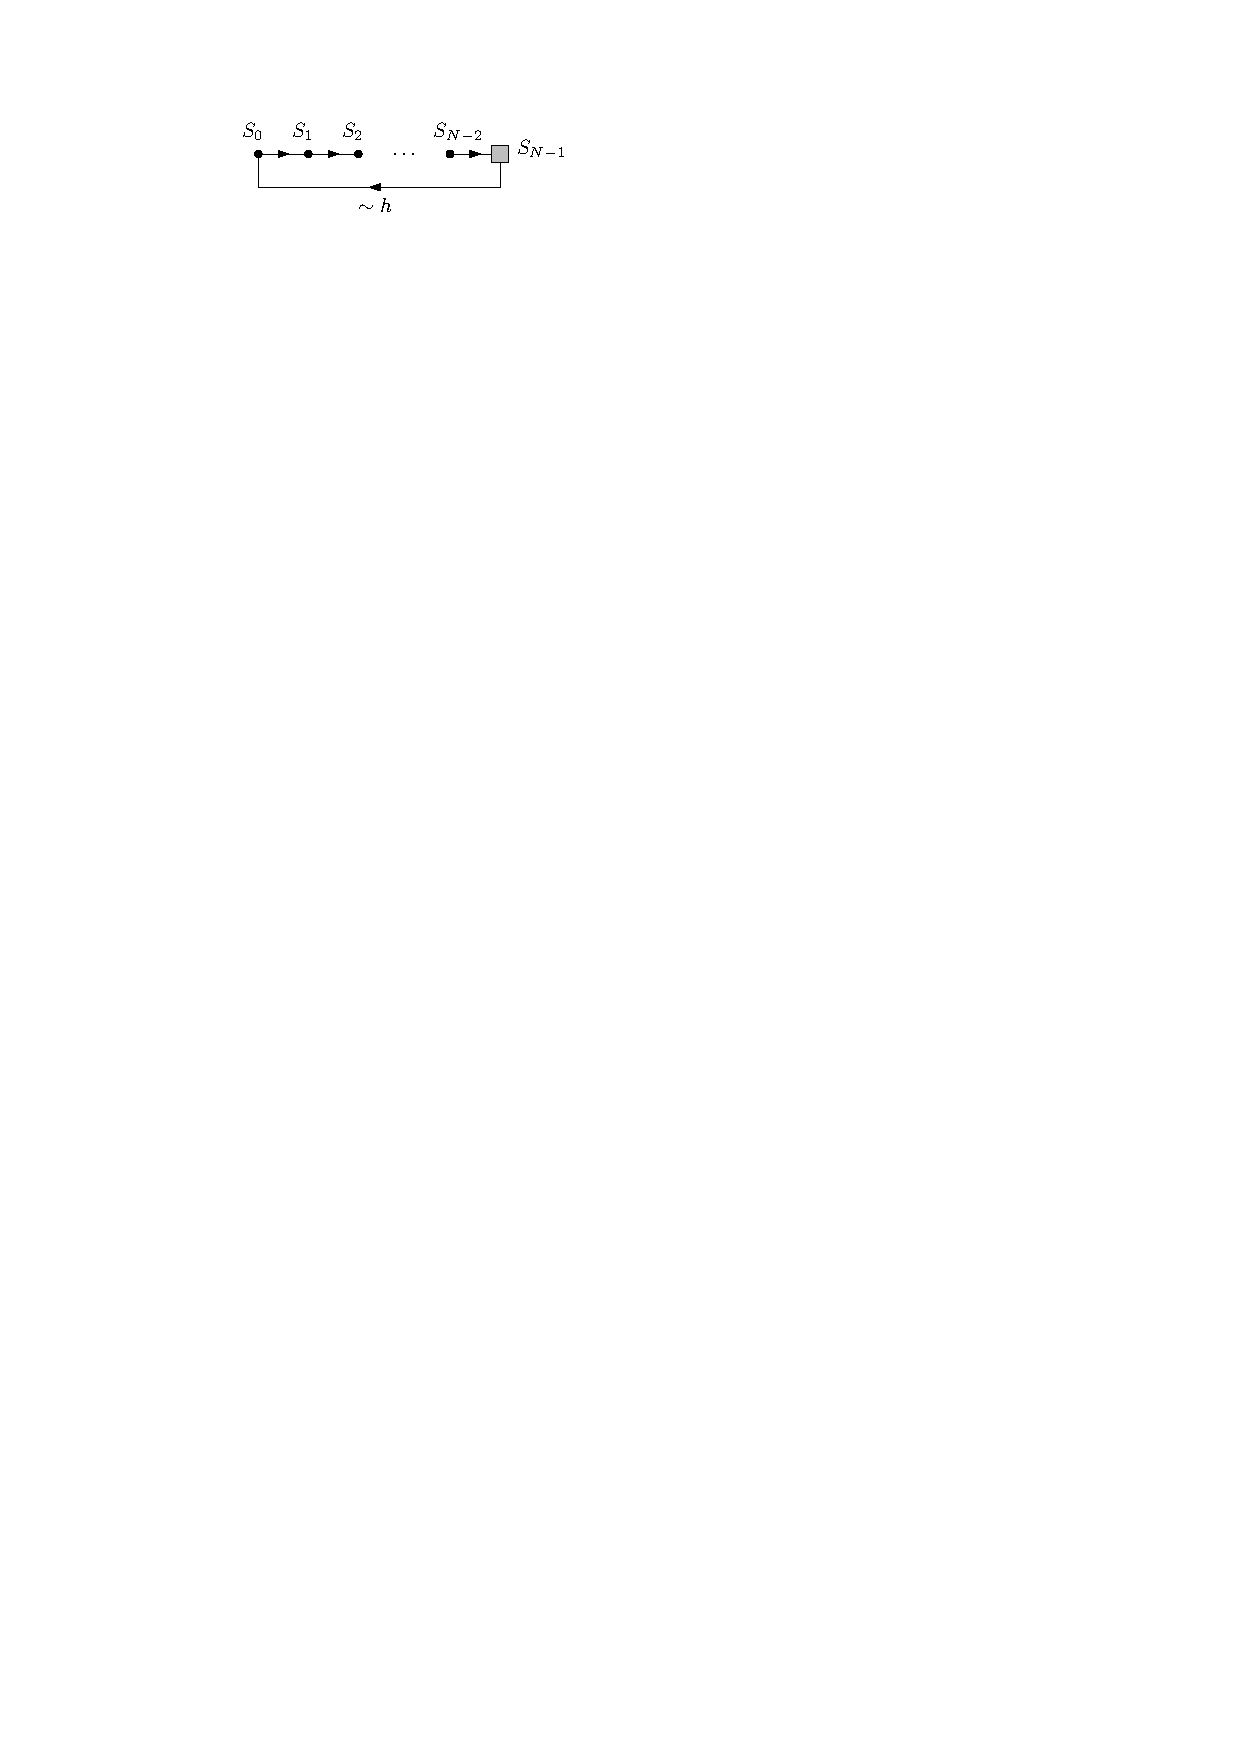
\includegraphics[width=0.4\textwidth]{figures/episodic_markov_chain.pdf}
  \caption{Illustration of the induced Markov chain when dealing with finite
    episodes. The next state after the final state, indicated as the grey
    rectangle, is sampled according to initial state distribution $h$.}
  \label{fig:episodic_MC}
\end{figure}

\subsection{Monte Carlo sampling}

Suppose we have some function $f : \mathcal{S} \rightarrow \mathbb{R}$ over
states and we are interested in estimating $\mathbb{E}_{S_{t}^{(i)} \sim \mu}[f(S_{t}^{(i)})]$.
%
We can just take random samples of $S_{t}^{(i)}$, by sampling initial state
$S_{0}^{(i)} \sim h$ and then \textit{rolling out} $\pi$ to obtain
$\tau^{(i)} = (S_{0}^{(i)},A_{0}^{(i)},R_{1}^{(i)},S_{1}^{(i)},A_{1}^{(i)},R_{2}^{(i)},S_{2}^{(i)}, \dots, S_{N^{(i)}-1}^{(i)}) \sim \pi(\tau^{(i)} | S_{0}^{(i)})$,
where $N^{(i)}$ denotes the total number of states visited in this episode.
%
Given $M$ such episode samples, we compute the estimate as
\begin{align*}
  \mathbb{E}_{S_{t}^{(i)} \sim \mu} [ f(S_{t}^{(i)}) ] \approx \left( \sum_{i=1}^{M} \sum_{t=0}^{N^{(i)} - 1} f(S_{t}^{(i)}) \right) / \left( \sum_{i=1}^{M} N^{(i)} \right) .
\end{align*}

Observe that the analysis of the induced Markov chain can be extended to
explicitly include actions and rewards as part of the state and derive the
stationary distribution of the resulting Markov chain. However, we do not need
this distribution explicitly in practice, because we can again use episode
samples $\tau^{(i)}$. To keep notation concise, we will from now on denote this
type of expectation as $\mathbb{E}_{\tau \sim h,\pi}[f(\tau)]$ and omit episode
superscripts.
%
Using this new notation, note that the average episode length is given by
\begin{align*}
  \mathbb{E}_{h, \pi} [ N ]= \sum_{s'} \eta(s') .
\end{align*}

\section{Policy gradient estimation}

Let $v_{\pi_{\theta}} = \mathbb{E}_{h,\pi_{\theta}}[G_{0}]$ denote the expected
episodic reward under policy $\pi$, where $G_{t}$ is called the reward-to-go at
step $t$, which is defined as
\begin{align*}
  G_{t} := \sum_{k=t+1}^{\infty} R_{k} .
\end{align*}
The main idea of policy gradient methods is to update the policy parameters
$\theta$ in the direction that increases the expected episodic reward the most. This
means that the policy parameters are updated as
\begin{align*}
  \theta_{k+1} = \theta_{k} + \alpha \nabla v_{\pi_{\theta}} ,
\end{align*}
where $\alpha$ is the learning rate and the gradient is with respect to
$\theta$. Instead of trying to derive or compute the gradient exactly, we often
use some statistical estimate based on sampled episode. The basic policy
gradient algorithm is to repeat the following three steps:

\vspace{1em}
\noindent
\texttt{repeat:\\
1. sample $M$ episodes $\tau^{(1)}, \dots, \tau^{(M)}$ following $\pi_{\theta}$\\
2. compute gradient estimate $\widehat{\nabla v_{\pi_{\theta}}}(\tau^{(1)}, \dots, \tau^{(M)})$\\
3. update $\theta \leftarrow \theta + \alpha \widehat{\nabla v_{\pi_{\theta}}}$
}

\subsection{Policy gradient theorem and REINFORCE estimator}

We will now present the fundamental policy gradient theorem, which essentially
provides a function $f$ such that
\begin{align*}
  \nabla v_{\pi_{\theta}} = \mathbb{E}_{\tau \sim h,\pi_{\theta}}[f(\tau)] ,
\end{align*}
which allows us to estimate the policy gradient using episode samples.
%
To align with the notation
of~\cite{suttonReinforcementLearningIntroduction2018}, we write
$\mathrm{Pr}(x \rightarrow s, k, \pi) := (Q^{k})_{xs}$, for the probability of
reaching state $s$ in $k$ steps under policy $\pi$, starting from state some
$x$, so that the expected number of visits can also be written as
\begin{align*}
  \eta(s) = \sum_{x} h(x) \sum_{k=0}^{\infty} \mathrm{Pr}(x \rightarrow s, k, \pi)
\end{align*}
%
As proven in the chapter on policy gradient methods
in~\cite{suttonReinforcementLearningIntroduction2018}, the gradient of the value
function for a fixed initial state $s_0$ with respect to the parameters is given
by
\begin{align}
  \nabla v_{\pi}(s_{0}) = \sum_{s} \sum_{k=0}^{\infty} \mathrm{Pr}(s_{0} \rightarrow s, k, \pi) \sum_{a} q_{\pi}(s,a) \nabla \pi(a|s) .
\end{align}
When choosing the initial state $s_{0}$ according to some distribution
$h(s_{0})$, we verify that the final result is still the same as in
\cite{suttonReinforcementLearningIntroduction2018}:
\begin{subequations}
\begin{align}
  \nabla v_{\pi} :=& \nabla \mathbb{E}_{s_{0} \sim h}[v_{\pi}(s_{0})] \\
  =& \sum_{s_{0}} h(s_{0}) \sum_{s} \sum_{k=0}^{\infty} \mathrm{Pr}(s_{0} \rightarrow s, k, \pi) \sum_{a} q_{\pi}(s,a) \nabla \pi(a|s) \\
  =& \sum_{s} \eta(s) \sum_{a} q_{\pi}(s,a) \nabla \pi(a|s) \\
  =& \sum_{s'} \eta(s') \sum_{s} \mu(s) \sum_{a} q_{\pi}(s,a) \nabla \pi(a|s) \\
  \propto& \sum_{s} \mu(s) \sum_{a} q_{\pi}(s,a) \nabla \pi(a|s) ,
\end{align}
\end{subequations}
where the constant of proportionality is just the average episode length.
%
Because we do not know $\mu$ or $q_{\pi}$ explicitly, we would like to estimate
$\nabla v_{\pi}$ based on samples. If we sample episodes according to $h$ and
$\pi$ as explained above, we encounter states according to $\mu$, so we have
\begin{subequations}
\begin{align}
  \nabla v_{\pi} &\propto \mathbb{E}_{h, \pi} \left[ \sum_{a} q_{\pi}(S_{t}, a) \nabla\pi(a | S_{t}) \right] \\
  &= \mathbb{E}_{h, \pi} \left[ \sum_{a} \pi(a | S_{t}) q_{\pi}(S_{t}, a) \frac{\nabla \pi(a | S_{t})}{\pi(a | S_{t})} \right] \\
  &= \mathbb{E}_{h, \pi} \left[ q_{\pi}(S_{t}, A_{t}) \frac{\nabla \pi(A_{t} | S_{t})}{\pi(A_{t}| S_{t})} \right] \\
  &= \mathbb{E}_{h, \pi} \left[ G_{t} \nabla \log \pi(A_{t} | S_{t}) \right] .
  \label{eq:estimator1}
\end{align}
\end{subequations}

\subsection{Baseline}
Let $b(s)$ be some function of the state $s$ only, then we have for any $s \in \mathcal{S}$
\begin{align}
  \sum_{a} b(s) \nabla \pi(a | s) = b(s) \nabla \sum_{a} \pi(a | s) = b(s) \nabla 1 = 0 .
\end{align}
This yields the so-called REINFORCE estimate with \textit{baseline}
\begin{subequations}
\begin{align}
  \nabla v_{\pi} &\propto \sum_{s} \mu(s) \sum_{a} (q_{\pi}(s, a) + b(s)) \nabla \pi(a | s) \\
          &= \mathbb{E}_{h, \pi} \left[ \bigl(q_{\pi}(S_{t}, A_{t}) + b(S_{t}) \bigr) \nabla \log \pi(A_{t} | S_{t}) \right] \\
  &= \mathbb{E}_{h, \pi} \left[ \bigl(G_{t} + b(S_{t}) \bigr) \nabla \log \pi(A_{t} | S_{t}) \right] .
  \label{eq:estimator2}
          %&= \mathbb{E}_{h, \pi} \left[ \bigl(G_{t} + b(S_{t}) \bigr) \nabla \log \pi(A_{t} | S_{t}) \right]
\end{align}
\end{subequations}
%
Although estimates~\eqref{eq:estimator1} and~\eqref{eq:estimator2} are both equivalent in terms of their expected
value, they may differ in higher moments, which is why an appropriate choice of
$b$ can make a lot of difference in how well the policy gradient algorithm
converges to an optimal policy.
%
As a specific baseline, consider the expected cumulative sum of rewards up to
step the current step $t$, defined as
\begin{align}
  b(s) = \mathbb{E}_{h,\pi} \left[ \sum_{k=1}^{t} R_{k} \Big| S_{t} = s \right],
\end{align}
then observe that
\begin{subequations}
\begin{align}
  q_{\pi}(s, a) + b(s) &= \mathbb{E}_{h,\pi}\left[ \sum_{k=t+1}^{\infty} R_{k} \Big| S_{t} = s , A_{t} = a \right] + \mathbb{E}_{h,\pi}\left[ \sum_{k=1}^{t} R_{k} \Big| S_{t} = s \right] \\
                     &= \mathbb{E}_{h,\pi}\left[ \sum_{k=1}^{\infty}  R_{k} \Big| S_{t} = s, A_{t} = a \right] \\
                     &= \mathbb{E}_{h,\pi} [ G_{0} | S_{t} = s, A_{t} = a ] ,
\end{align}
\end{subequations}
which is just the expected total episodic reward.
%
Now define function $f$ to be
\begin{subequations}
\begin{align}
  f(s, a) := (q_{\pi}(s, a) + b(s))\nabla \log \pi(a | s) &= \mathbb{E}_{h,\pi} \left[ G_{0} | S_{t} = s, A_{t} = a \right] \nabla \log \pi(a | s) \\
  &= \mathbb{E}_{h,\pi} \left[ G_{0} \nabla \log \pi(a | s) | S_{t} = s, A_{t} = a \right] ,
\end{align}
\end{subequations}
then applying the law of total expectation yields
\begin{align}
  \nabla v_{\pi} \propto \mathbb{E}_{h,\pi}[f(S_{t}, A_{t})] =  \mathbb{E}_{h, \pi} \left[ G_{0} \nabla \log \pi(A_{t} | S_{t}) \right] .
\end{align}




\bibliography{references}
\bibliographystyle{ieeetr}

\end{document}
